\documentclass{article}

\usepackage{graphicx}
\usepackage[utf8]{inputenc}
\usepackage[T1]{fontenc}
\usepackage[francais]{babel}
\usepackage{hyperref}
\usepackage{amsmath,amsfonts,amssymb}
\usepackage{Tkz-Tab}
\usepackage{wrapfig}
\usepackage{Verbatim}

\begin{document}

\title{L'algue tueuse
	\smallbreak
	TD n\degre3
	\smallbreak
	Modélisation mathématique
	\smallbreak
	Q4}
\author{Sibylle Roux \and Juliette Arazo \and Nicolas Le Gallo \and Tanguy Thomas}


\maketitle

\newpage

\tableofcontents

\newpage

\section{Etude du modèle logistique avec effet Allee et immigration}

\subsection{Etude numérique}

\subsubsection{Modèle avec variation de I}

\paragraph{Courbe de la vitesse d'accroissement}
\begin{center}
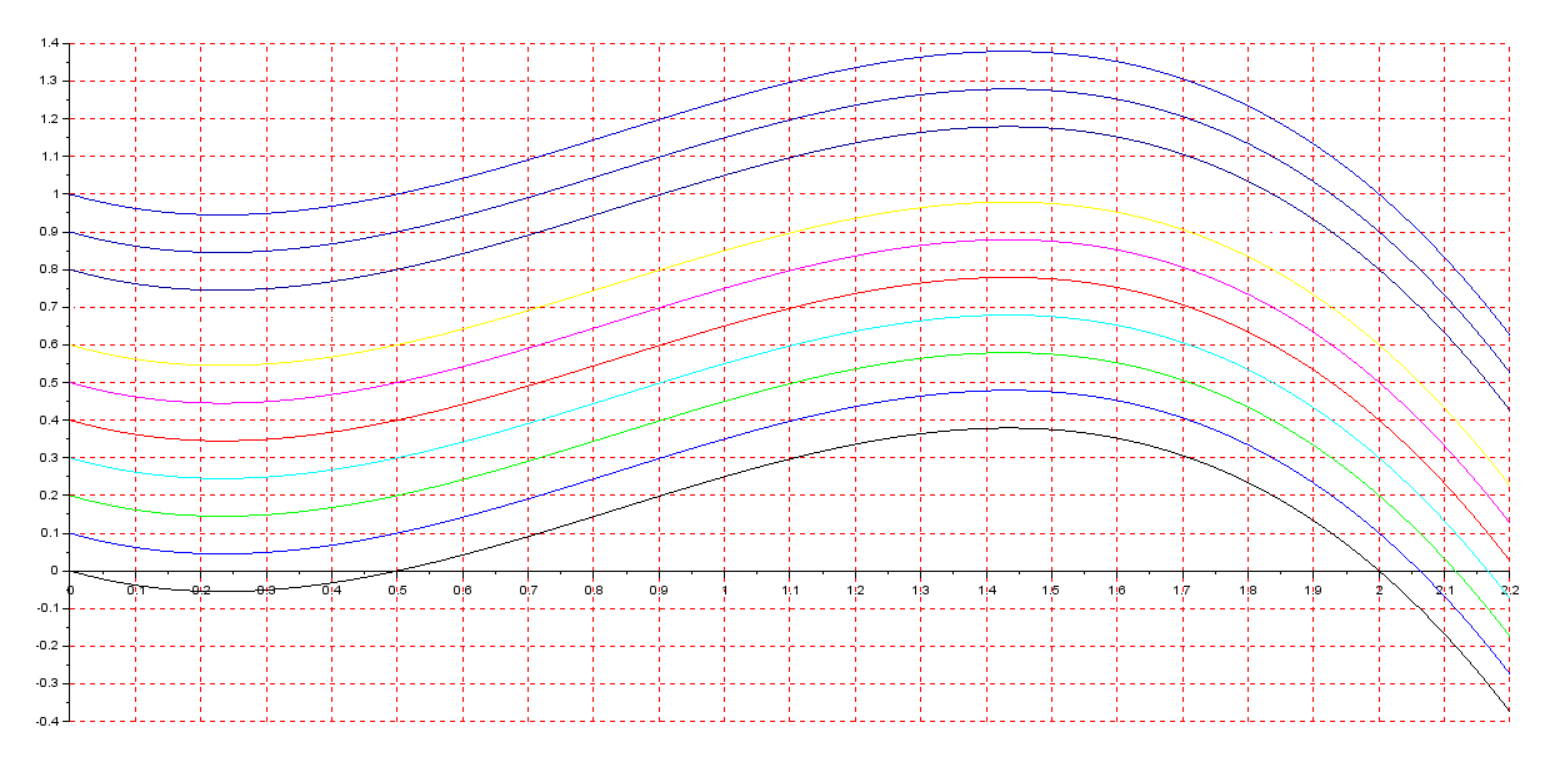
\includegraphics[width=300px]{img/part1/AlleeI.png}
\end{center}
Paramètres de modélisation : $K=2$  ; $r=0.5$ ; $A=0.5$ ; $I$ varie de 0 à 1 avec un pas de 0.1 
\paragraph{}

\newpage

\paragraph{Discrétisation du modèle}
\begin{center}
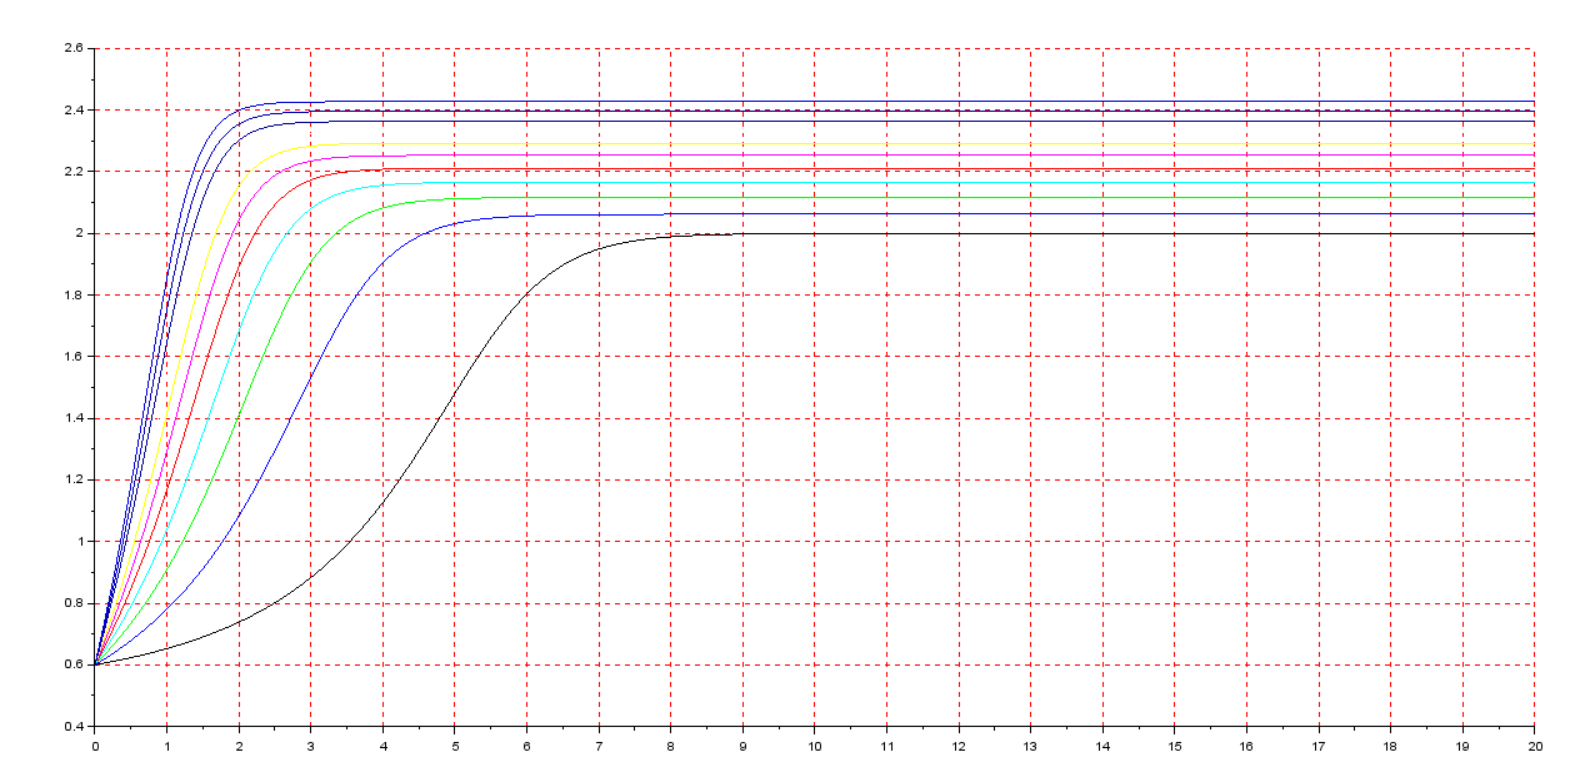
\includegraphics[width=300px]{img/part1/TrajI.png}
\end{center}
Paramètres de modélisation : $a=0.6$ ; $K=2$  ; $r=0.5$ ; $A=0.5$ ; $I$ varie de 0 à 1 avec un pas de 0.1
\paragraph{}

\subsubsection{Modèle avec variation de K}

\paragraph{Courbe de la vitesse d'accroissement}
\begin{center}
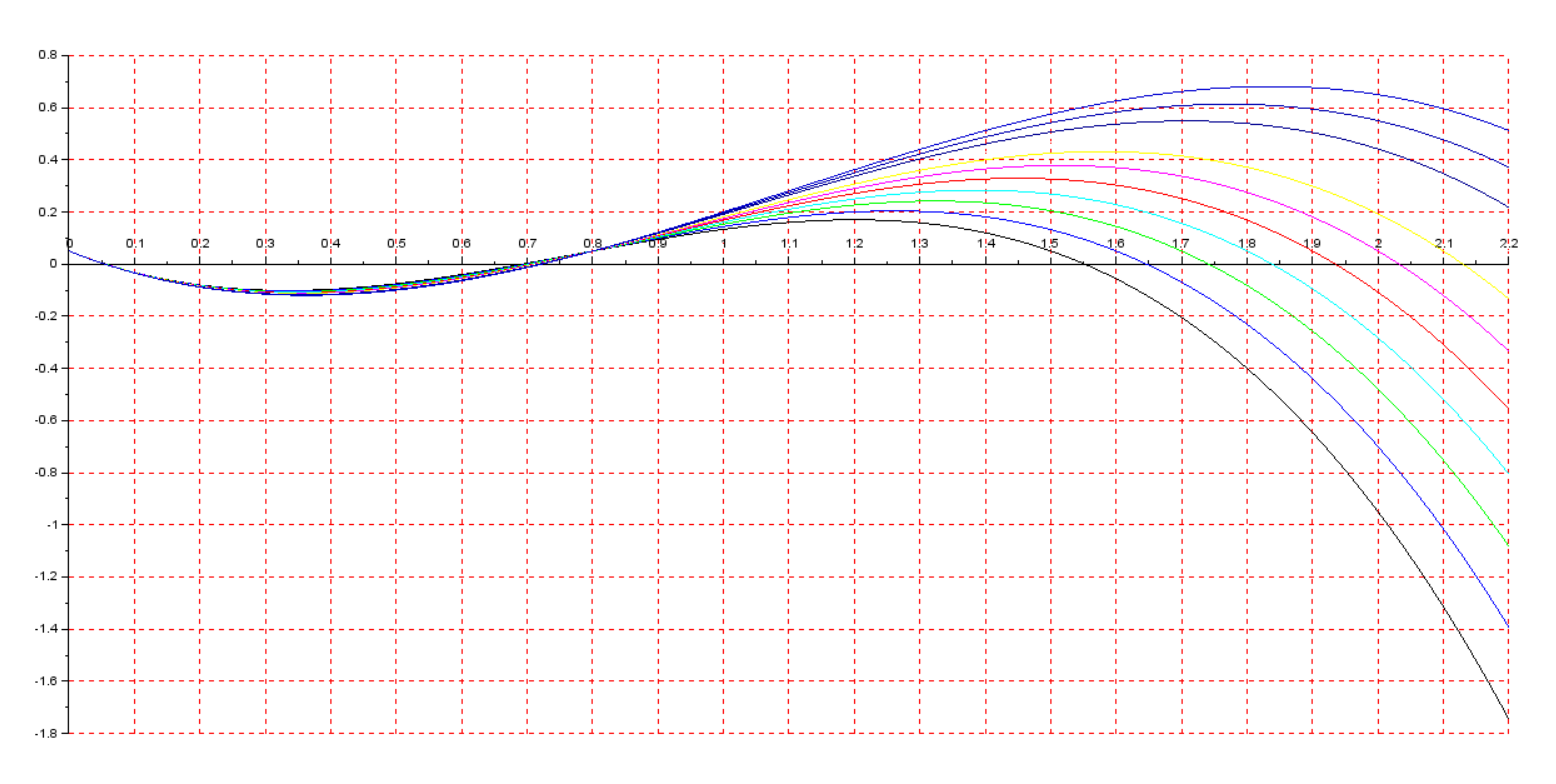
\includegraphics[width=300px]{img/part1/AlleeK.png}
\end{center}
Paramètres de modélisation : $r=1$ ; $A=0.8$ ; $I=0.05$ ; $K$ varie de 1.5 à 2.5 avec un pas de 0.1
\paragraph{}

\paragraph{Discrétisation du modèle}
\begin{center}
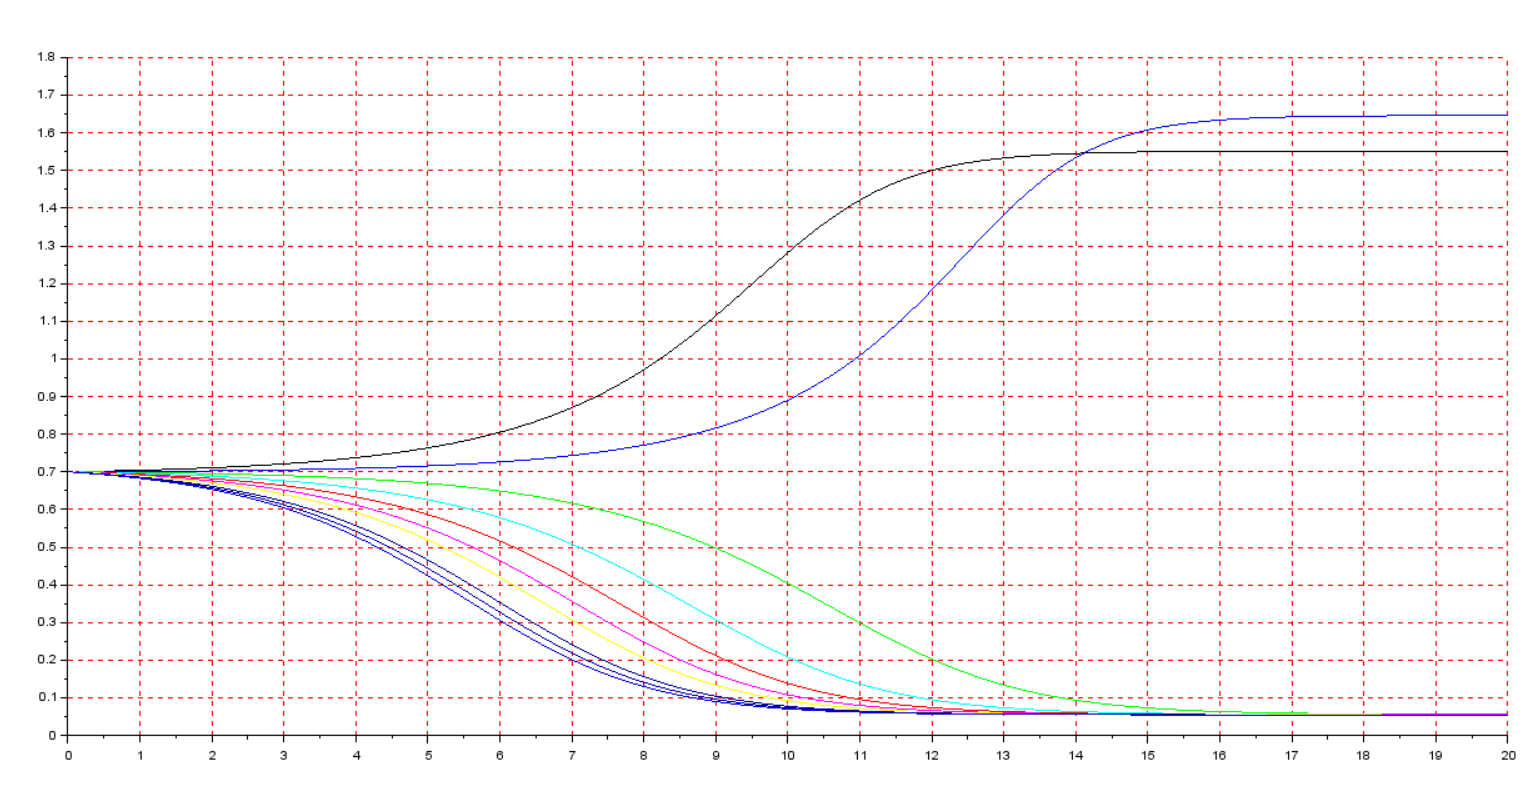
\includegraphics[width=300px]{img/part1/TrajK.png}
\end{center}
Paramètres de modélisation : $a=0.7$ ; $r=1$ ; $A=0.8$ ; $I=0.05$ ; $K$ varie de 1.5 à 2.5 avec un pas de 0.1
\paragraph{}

\subsubsection{Modèle avec variation de A}

\paragraph{Courbe de la vitesse d'accroissement}
\begin{center}
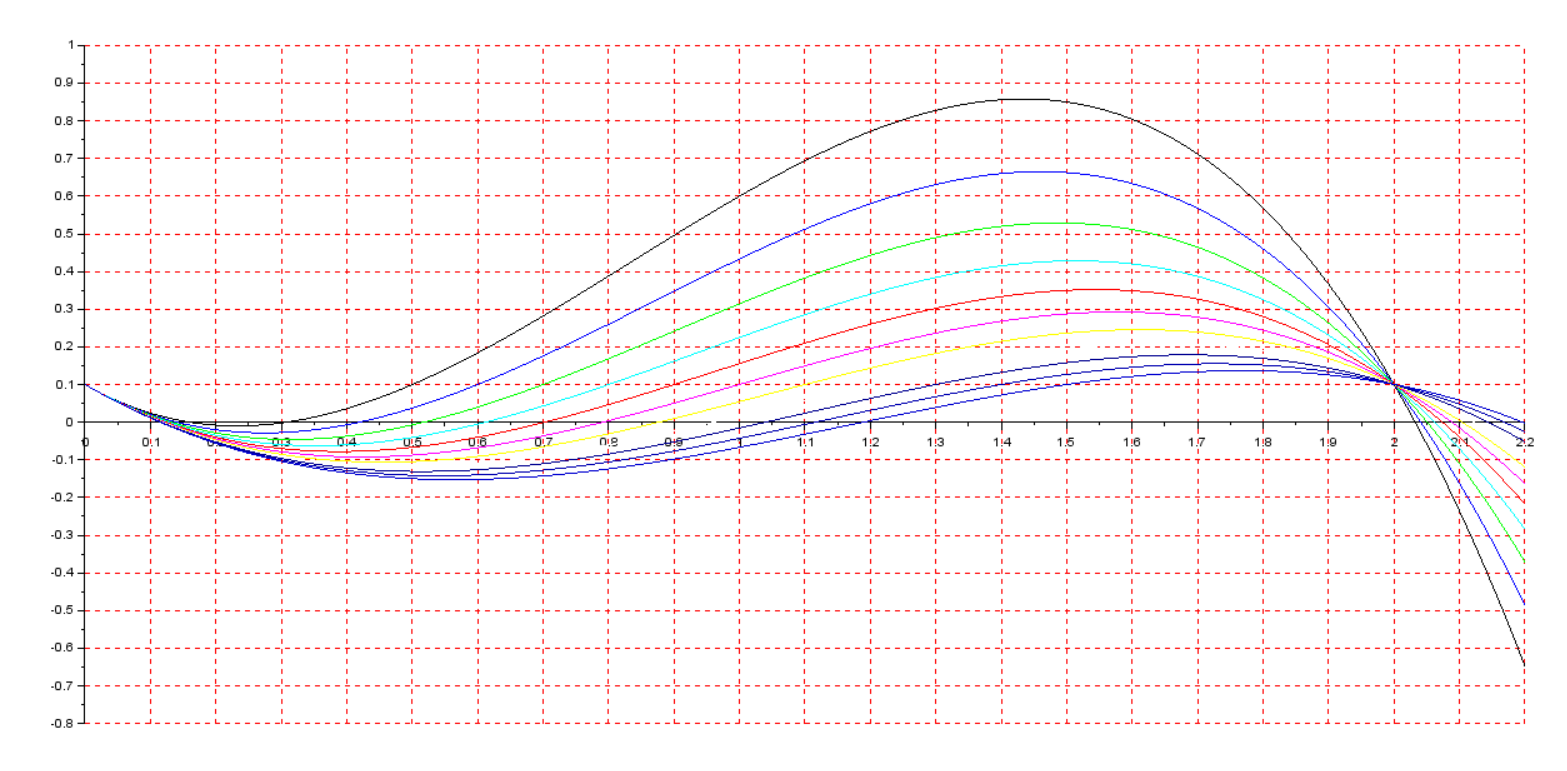
\includegraphics[width=300px]{img/part1/AlleeA.png}
\end{center}
Paramètres de modélisation : $I=0.1$ ; $K=2$ ; $r=1$  ; $A$ varie de 0.5 à 1.5 avec un pas de 0.1
\paragraph{}

\paragraph{Discrétisation du modèle}
\begin{center}
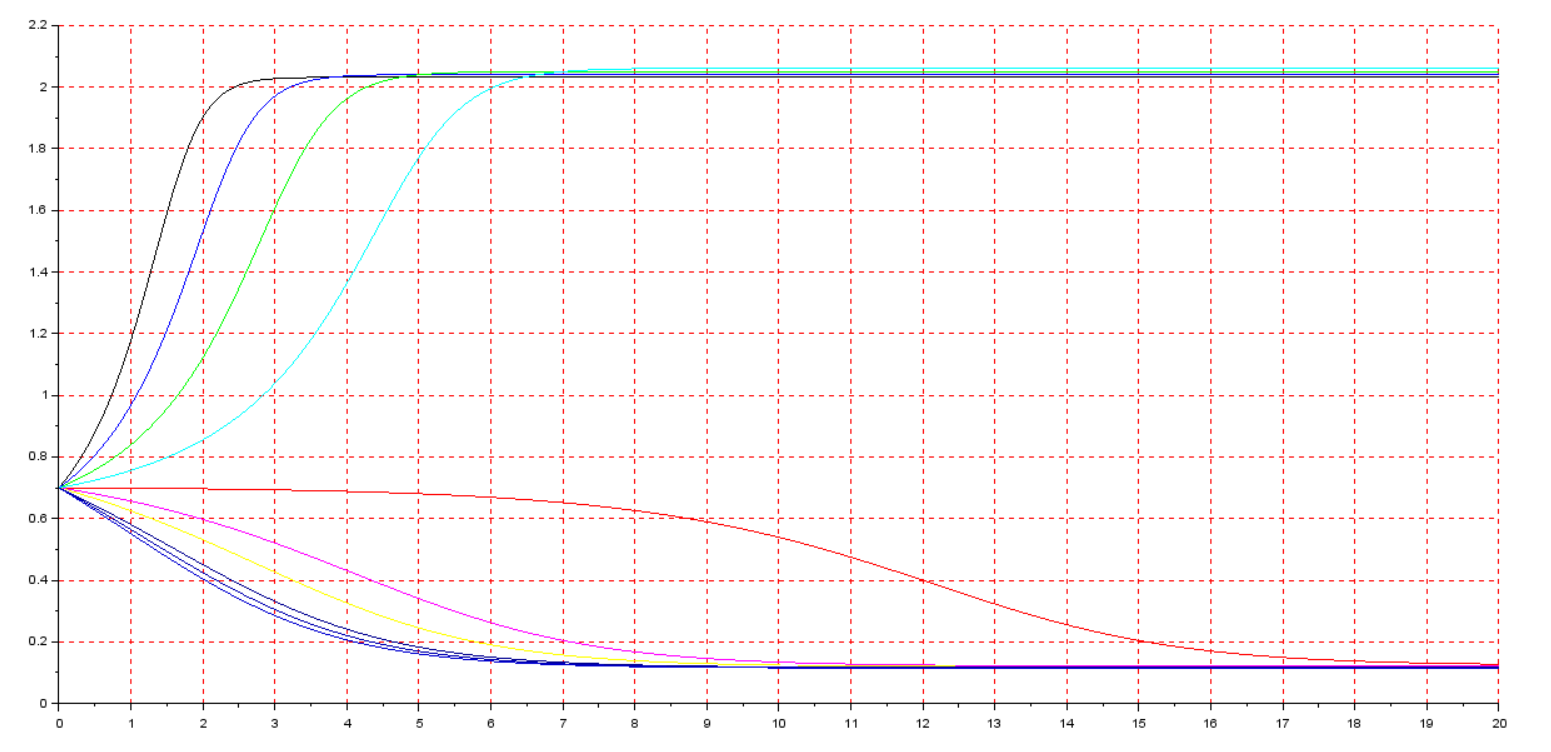
\includegraphics[width=300px]{img/part1/TrajA.png}
\end{center}
Paramètres de modélisation : $a=0.7$ ; $I=0.1$ ; $K=2$ ; $r=1$  ; $A$ varie de 0.5 à 1.5 avec un pas de 0.1
\paragraph{}

\subsubsection{Modèle avec variation de la population initiale}

\paragraph{Discretisation du modèle}
\begin{center}
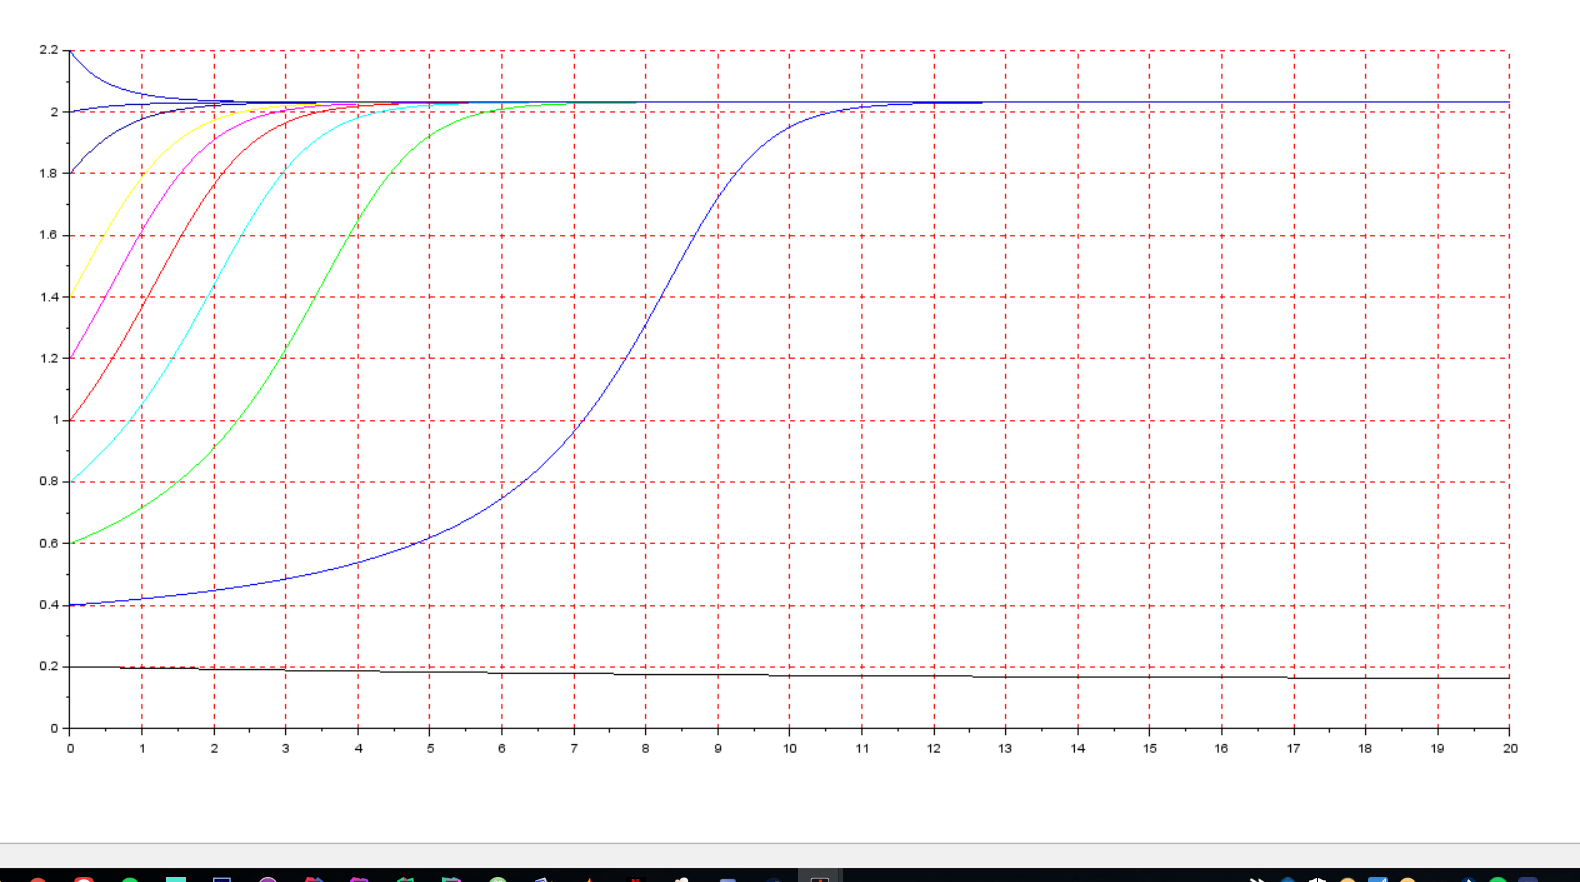
\includegraphics[width=300px]{img/part1/TrajPop.png}
\end{center}
Paramètres de modélisation : $A=0.5$ ; $I=0.1$ ; $K=2$ ; $r=0.25$  ; $a$ varie de 0.5 à 1.5 avec un pas de 0.1
\paragraph{}

\newpage

\subsection{Etude mathématique}


\subsection{Bilan}
\paragraph{}

\newpage
\section{Etude du modèle logistique avec prédation}

\subsection{Etude numérique}

\subsubsection{Modèle logistique}

\paragraph{Vitesse d'accroissement}
\begin{center}
%\includegraphics[width=300px]{allee.png}
\end{center}
Paramètres de modélisation : 
\paragraph{}

\paragraph{Discretisation}
\begin{center}
%\includegraphics[width=300px]{discretisationAllee.png}
\end{center}
Paramètres de modélisation : 
\paragraph{}

\subsubsection{Modèle logistique}
\begin{center}
%\includegraphics[width=300px]{discretisationAlleea.PNG}
\end{center}
Paramètres de modélisation :
\paragraph{}

\subsubsection{Modèle logistique}
\begin{center}
%\includegraphics[width=300px]{discretisationAlleeK.PNG}
\end{center}
Paramètres de modélisation : 
\paragraph{}

\subsubsection{Modèle logistique}
\begin{center}
%\includegraphics[width=300px]{discretisationAlleeSeuil.PNG}
\end{center}
Paramètres de modélisation : 
\paragraph{}

\subsection{Etude mathématique}

\subsection{Bilan}
\paragraph{}


\newpage
\appendix

\section{Etude du modèle logistique avec effet Allee et immigration- Scripts Scilab}

\subsection{Modèle avec variation de I}

\subsubsection{Vitesse d'accroissement}

\begin{verbatim}
clear
clf

r = 0.5 ; A = 0.5 ; K = 2 ; // variables du modèles
Ivect=0:0.1:1; // variable qui varie
x = linspace(0, 2.2, 301); // vecteur contenant les valeurs de la vitesse d'accroissement

function f = allee_imig(x) // fonction qui calcule la vitesse d'accroissement
    f = r * x .* (x / A - 1 ) .* (1 - x / K)+ I // opérations vectorielles. x est un vecteur
endfunction

for i=1:11; // Bouclae qui va dessiner les différentes courbes
    I=Ivect(i); // vecteur contenant les différentes valeurs de I
    plot2d(x, allee_imig(x), style = i) // Tracé de la vitesse d'accroissement
end

// Définition des paramètres d'affichages
a=gca();
a.x_location = "origin";
a.grid=[5,5];
\end{verbatim}

\subsubsection{Discretisation}

\begin{verbatim}
clear
clf

Ivect=0:0.1:1; // variable qui varie
r = 0.5 ; A = 0.5 ; K = 2 ; h = 0.05 ; a = 0.6 ; // variables du modèles + pas de temps
ndate = 0:h:20; // vecteur des instants où on calcule la solution

function f = allee_img(x) // fonction qui calcule la vitesse d'accroissement
    f = r * x .* (x / A - 1 ) .* (1 - x / K)+I // opérations vectorielles. x est un vecteur
endfunction

x(1)=a; // Initialisation de la population initiale

for i=1:11; // Boucle qui va dessiner les différentes courbes
    I=Ivect(i); // vecteur contenant les différentes valeurs de I
    for n = 1:length(ndate) - 1 // Boucle qui calcule la courbe de la population
        x(n+1) = x(n) + h * allee_img(x(n)); // Calcul de la population
    end 
    plot2d(ndate, x, style = i) // Tracé de la discretisation
end

// Définition des paramètres d'affichages
a=gca();
a.x_location = "origin";
a.grid=[5,5];
\end{verbatim}

\subsection{Modèle avec variation de K}

\subsubsection{Vitesse d'accroissement}

\begin{verbatim}
clear
clf

r = 1 ; A = 0.8 ; I=0.05 ; // variables du modèles
Kvect=1.5:0.1:2.5; // variable qui varie
x = linspace(0, 2.2, 301); // vecteur contenant les valeurs de la vitesse d'accroissement

function f = allee_imig(x) // fonction qui calcule la vitesse d'accroissement
    f = r * x .* (x / A - 1 ) .* (1 - x / K)+ I // opérations vectorielles. x est un vecteur
endfunction

for i=1:11; // Boucle qui va dessiner les différentes courbes
    K=Kvect(i); // vecteur contenant les différentes valeurs de K
    plot2d(x, allee_imig(x), style = i) // Tracé de la vitesse d'accroissement
end

// Définition des paramètres d'affichages
a=gca();
a.x_location = "origin";
a.grid=[5,5];
\end{verbatim}

\subsubsection{Discretisation}

\begin{verbatim}
clear
clf

Kvect=1.5:0.1:2.5; // variable qui varie
r = 1 ; A = 0.8 ; I=0.05 ; h = 0.05 ; a = 0.7 ; // variables du modèles + pas de temps
ndate = 0:h:20; // vecteur des instants où on calcule la solution

function f = allee_img(x) // fonction qui calcule la vitesse d'accroissement
    f = r * x .* (x / A - 1 ) .* (1 - x / K)+I // opérations vectorielles. x est un vecteur
endfunction

x(1)=a; // Initialisation de la population initiale

for i=1:11; // Boucle qui va dessiner les différentes courbes
    K=Kvect(i); // vecteur contenant les différentes valeurs de K
    for n = 1:length(ndate) - 1 // Boucle qui calcule la courbe de la population
        x(n+1) = x(n) + h * allee_img(x(n)); // Calcul de la population
    end 
    plot2d(ndate, x, style = i) // Tracé de la discretisation
end

// Définition des paramètres d'affichages
a=gca();
a.x_location = "origin";
a.grid=[5,5];
\end{verbatim}

\subsection{Modèle avec variation de A}

\subsubsection{Vitesse d'accroissement}

\begin{verbatim}
clear
clf

r = 1 ; K = 2 ; I=0.1 ; // variables du modèles
Avect=0.5:0.1:1.5; // variable qui varie
x = linspace(0, 2.2, 301); // vecteur contenant les valeurs de la vitesse d'accroissement

function f = allee_imig(x) // fonction qui calcule la vitesse d'accroissement
    f = r * x .* (x / A - 1 ) .* (1 - x / K)+ I // opérations vectorielles. x est un vecteur
endfunction

for i=1:11; // Boucle qui va dessiner les différentes courbes
    A=Avect(i); // vecteur contenant les différentes valeurs de A
    plot2d(x, allee_imig(x), style = i) // Tracé de la vitesse d'accroissement
end

// Définition des paramètres d'affichages
a=gca();
a.x_location = "origin";
a.grid=[5,5];
\end{verbatim}

\subsubsection{Discretisation}

\begin{verbatim}
clear
clf

Avect=0.5:0.1:1.5; // variable qui varie
r = 1 ; K = 2 ; I=0.1 ; h = 0.05 ; a = 0.7 ; // variables du modèles + pas de temps
ndate = 0:h:20; // vecteur des instants où on calcule la solution

function f = allee_img(x) // fonction qui calcule la vitesse d'accroissement
    f = r * x .* (x / A - 1 ) .* (1 - x / K)+I // opérations vectorielles. x est un vecteur
endfunction

x(1)=a; // Initialisation de la population initiale

for i=1:11; // Boucle qui va dessiner les différentes courbes
    A=Avect(i); // vecteur contenant les différentes valeurs de A
    for n = 1:length(ndate) - 1 // Boucle qui calcule la courbe de la population
        x(n+1) = x(n) + h * allee_img(x(n)); // Calcul de la population
    end 
    plot2d(ndate, x, style = i) // Tracé de la discretisation
end

// Définition des paramètres d'affichages
a=gca();
a.x_location = "origin";
a.grid=[5,5];
\end{verbatim}

\subsection{Modèle avec variation de la population initiale}

\begin{verbatim}
clear
clf

avect=0.5:0.1:1.5; // variable qui varie
r = 0.25 ; K = 2 ; I=0.1 ; A = 0.5 ; h = 0.05 ; // variables du modèles + pas de temps
ndate = 0:h:20; // vecteur des instants où on calcule la solution

function f = allee_img(x) // fonction qui calcule la vitesse d'accroissement
    f = r * x .* (x / A - 1 ) .* (1 - x / K)+I // opérations vectorielles. x est un vecteur
endfunction

for i=1:11; // Boucle qui va dessiner les différentes courbes
    x(1)=avect(i); // vecteur contenant les différentes valeurs de a
    for n = 1:length(ndate) - 1 // Boucle qui calcule la courbe de la population
        x(n+1) = x(n) + h * allee_img(x(n)); // Calcul de la population
    end 
    plot2d(ndate, x, style = i) // Tracé de la discretisation
end

// Définition des paramètres d'affichages
a=gca();
a.x_location = "origin";
a.grid=[5,5];
\end{verbatim}

\section{Etude du modèle logistique avec prédation - Scripts Scilab}

\subsection{Modèle logistique}

\subsubsection{Vitesse d'accroissement}

\begin{verbatim}
\end{verbatim}

\subsubsection{Discretisation}

\begin{verbatim}
\end{verbatim}

\subsection{Modèle logistique}

\begin{verbatim}
\end{verbatim}

\subsection{Modèle logistique}

\begin{verbatim}
\end{verbatim}

\subsection{Modèle logistique}

\begin{verbatim}
\end{verbatim}

\end{document}